\chapter{Week 3 - Topological Properties of Domains and Conservative Vector Fields}

\subsection{Connectivity and Simply Connected Domains}

\begin{definition}{Convex Domain}{def:convex_domain}
A domain $\Omega \subset \mathbb{R}^n$ is \textbf{convex} if for every pair of points $x, y \in \Omega$, the line segment joining $x$ and $y$ is entirely contained in $\Omega$[cite: 1]:
\[
[x, y] = \{ (1-t)x + ty \mid t \in [0, 1] \} \subset \Omega.
\]
If a domain is convex, then it is connected[cite: 1]. However, the converse is false in general: a connected domain is not necessarily convex[cite: 1].
\end{definition}

\begin{center}
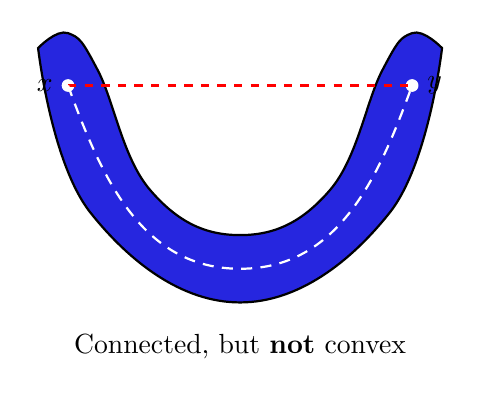
\begin{tikzpicture}[scale=0.95]
    % Non-convex but connected (U-shape domain)
    \draw[thick, fill=blue!85!black, fill opacity=0.85] 
        plot [smooth, tension=0.7] coordinates {
            (-2.7, 1.6) (-2.0, -0.6) (0, -1.8) (2.0, -0.6) (2.7, 1.6)
        }
        -- plot [smooth, tension=0.7] coordinates {
            (2.7, 1.6) (2.3, 1.8) (1.9, 1.3) (1.2, -0.3) (0, -0.9) (-1.2, -0.3) (-1.9, 1.3) (-2.3, 1.8) (-2.7, 1.6)
        } -- cycle;

    \coordinate (X) at (-2.3, 1.1);
    \coordinate (Y) at (2.3, 1.1);

    \filldraw[white] (X) circle (2.2pt) node[left=2pt, text=black] {$x$};
    \filldraw[white] (Y) circle (2.2pt) node[right=2pt, text=black] {$y$};

    % Line segment leaving the domain
    \draw[thick, red, dashed] (X) -- (Y);

    % Path remaining inside the domain
    \draw[thick, white, dash pattern=on 4pt off 3pt] 
        (X) to[out=-70, in=180] (0, -1.35) to[out=0, in=-110] (Y);

    \node[below] at (0, -2.1) {Connected, but \textbf{not} convex};
\end{tikzpicture}
\end{center}

\begin{definition}{Simply Connected Domain}{def:simply_connected}
An open domain $\Omega \subset \mathbb{R}^n$ is \textbf{simply connected} if it is connected and if for all $x, y \in \Omega$ and any two curves $\Gamma_1, \Gamma_2 \subset \Omega$ joining $x$ to $y$, the curve $\Gamma_1$ can be continuously deformed into $\Gamma_2$ without leaving $\Omega$ (i.e., every closed loop in $\Omega$ can be continuously contracted to a point within $\Omega$)[cite: 1].
\end{definition}

\begin{center}
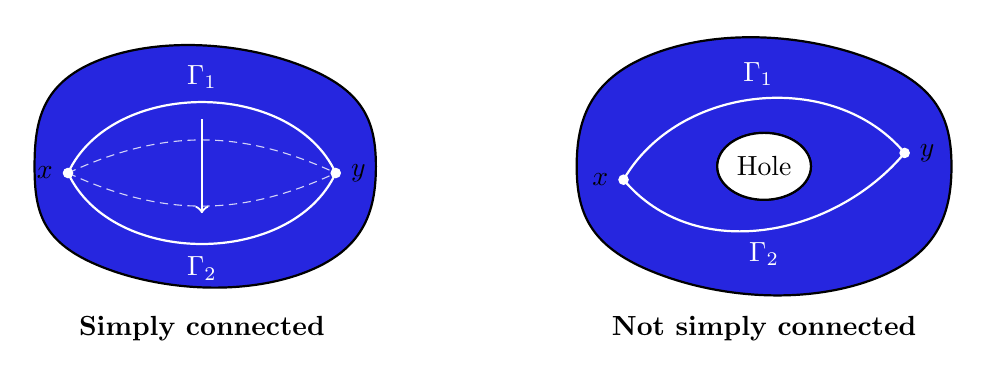
\begin{tikzpicture}[scale=0.85]
    % Simply connected domain
    \begin{scope}[shift={(-4.2, 0)}]
        \draw[thick, fill=blue!85!black, fill opacity=0.85] 
            plot [smooth cycle, tension=0.8] coordinates {(-2.5,0) (-1.5,1.6) (1.5,1.5) (2.6,0) (1.5,-1.6) (-1.5,-1.5)};
        
        \coordinate (X1) at (-2.0, -0.1);
        \coordinate (Y1) at (2.0, -0.1);
        \filldraw[white] (X1) circle (2pt) node[left=2pt, text=black] {$x$};
        \filldraw[white] (Y1) circle (2pt) node[right=2pt, text=black] {$y$};

        \draw[thick, white] (X1) to[out=65, in=115] node[midway, above=1pt] {$\Gamma_1$} (Y1);
        \draw[thick, white] (X1) to[out=-65, in=-115] node[midway, below=1pt] {$\Gamma_2$} (Y1);

        % Intermediate deformation curves
        \draw[white, dash pattern=on 3pt off 2pt, opacity=0.8] (X1) to[out=25, in=155] (Y1);
        \draw[white, dash pattern=on 3pt off 2pt, opacity=0.8] (X1) to[out=-25, in=-155] (Y1);
        \draw[->, thick, white] (0, 0.7) -- (0, -0.7);

        \node[below] at (0, -2.1) {\textbf{Simply connected}};
    \end{scope}

    % Non-simply connected domain (with a hole)
    \begin{scope}[shift={(4.2, 0)}]
        \draw[thick, fill=blue!85!black, fill opacity=0.85, even odd rule] 
            plot [smooth cycle, tension=0.8] coordinates {(-2.8,0) (-1.6,1.7) (1.6,1.6) (2.8,0) (1.6,-1.7) (-1.6,-1.6)}
            (0,0) ellipse (0.7cm and 0.5cm);

        \fill[white] (0,0) ellipse (0.69cm and 0.49cm);
        \draw[thick] (0,0) ellipse (0.7cm and 0.5cm);

        \coordinate (X2) at (-2.1, -0.2);
        \coordinate (Y2) at (2.1, 0.2);
        \filldraw[white] (X2) circle (2pt) node[left=2pt, text=black] {$x$};
        \filldraw[white] (Y2) circle (2pt) node[right=2pt, text=black] {$y$};

        \draw[thick, white] (X2) to[out=60, in=130] node[midway, above=1pt] {$\Gamma_1$} (Y2);
        \draw[thick, white] (X2) to[out=-50, in=-130] node[midway, below=1pt] {$\Gamma_2$} (Y2);

        \node at (0, 0) {Hole};
        \node[below] at (0, -2.1) {\textbf{Not simply connected}};
    \end{scope}
\end{tikzpicture}
\end{center}

---

\subsection{Characterization of Conservative Vector Fields}

\begin{theoreme}{Characterization of Conservative Fields}{thm:charac_conservative}
Let $\Omega \subset \mathbb{R}^n$ be an open connected domain, and let $F \colon \Omega \to \mathbb{R}^n$ be a continuous vector field ($F \in C^0(\Omega, \mathbb{R}^n)$)[cite: 1]. The following statements are equivalent:
\begin{enumerate}
    \item $F$ derives from a potential in $\Omega$ (i.e., there exists a $C^1$ scalar function $f$ such that $\nabla f = F$)[cite: 1].
    \item Path independence: for any pair of points $x, y \in \Omega$ and any two piecewise regular simple curves $\Gamma_1, \Gamma_2 \subset \Omega$ joining $x$ to $y$[cite: 1],
    \[
    \int_{\Gamma_1} F \cdot \mathrm{d}\ell = \int_{\Gamma_2} F \cdot \mathrm{d}\ell.
    \]
    \item For every piecewise regular closed simple curve $\Gamma \subset \Omega$[cite: 1],
    \[
    \oint_{\Gamma} F \cdot \mathrm{d}\ell = 0.
    \]
\end{enumerate}
\end{theoreme}

\begin{proof}
Let $\Gamma$ be the closed loop formed by concatenating $\Gamma_1$ and $-\Gamma_2$ (the curve $\Gamma_2$ traversed in the opposite direction from $y$ to $x$)[cite: 1]:
\[
\oint_{\Gamma} F \cdot \mathrm{d}\ell = \int_{\Gamma_1} F \cdot \mathrm{d}\ell + \int_{-\Gamma_2} F \cdot \mathrm{d}\ell = \int_{\Gamma_1} F \cdot \mathrm{d}\ell - \int_{\Gamma_2} F \cdot \mathrm{d}\ell.
\]
Thus[cite: 1]:
\[
\int_{\Gamma_1} F \cdot \mathrm{d}\ell = \int_{\Gamma_2} F \cdot \mathrm{d}\ell \iff \oint_{\Gamma} F \cdot \mathrm{d}\ell = 0. \qedhere
\]
\end{proof}

\begin{center}
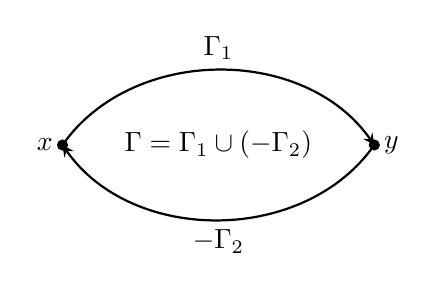
\begin{tikzpicture}[scale=0.9]
    \coordinate (X) at (-2.2, 0);
    \coordinate (Y) at (2.2, 0);
    \filldraw (X) circle (2pt) node[left] {$x$};
    \filldraw (Y) circle (2pt) node[right] {$y$};

    \draw[thick, -stealth] (X) to[out=55, in=125] node[midway, above] {$\Gamma_1$} (Y);
    \draw[thick, -stealth] (Y) to[out=-125, in=-55] node[midway, below] {$-\Gamma_2$} (X);

    \node at (0, 0) {$\Gamma = \Gamma_1 \cup (-\Gamma_2)$};
\end{tikzpicture}
\end{center}

---

\subsection{Summary of Conditions for Gradient Fields}

Let $\Omega \subset \mathbb{R}^n$ be an open domain and $F \in C^1(\Omega, \mathbb{R}^n)$ (with $n = 2$ or $3$)[cite: 1]:
\begin{enumerate}[label=(\alph*)]
    \item If $\operatorname{curl} F \neq 0$ at some point in $\Omega$, then $F$ does not derive from a potential in $\Omega$[cite: 1].
    \item If $\operatorname{curl} F = 0$ in $\Omega$, and $\Omega$ is \textbf{convex} (or \textbf{simply connected}), then $F$ derives from a potential in $\Omega$[cite: 1].
    \item If $\operatorname{curl} F = 0$ in $\Omega$, but $\Omega$ is \textbf{neither convex nor simply connected}, the integrability criterion is inconclusive without further information[cite: 1].
    \item If there exists a closed curve $\Gamma \subset \Omega$ such that $\oint_{\Gamma} F \cdot \mathrm{d}\ell \neq 0$, then $F$ does not derive from a potential in $\Omega$[cite: 1].
    \item If for a specific closed curve $\Gamma \subset \Omega$ we find $\oint_{\Gamma} F \cdot \mathrm{d}\ell = 0$, this does not imply that $F$ is conservative in general (the vanishing condition must hold for \emph{all} closed curves)[cite: 1].
\end{enumerate}

---

\subsection{Examples}

\subsubsection*{Example (a): 2D Vector Field}
Consider $F \colon \mathbb{R}^2 \to \mathbb{R}^2$ defined by[cite: 1]:
\[
F(x, y) = \big(4x^3 y^2,\, 2x^4 y + y\big).
\]
\textbf{1. Test for curl:}\\
The components are $F_1(x, y) = 4x^3 y^2$ and $F_2(x, y) = 2x^4 y + y$. Computing the partial derivatives:
\[
\frac{\partial F_2}{\partial x} = \frac{\partial}{\partial x}(2x^4 y + y) = 8x^3 y, \qquad \frac{\partial F_1}{\partial y} = \frac{\partial}{\partial y}(4x^3 y^2) = 8x^3 y.
\]
Since $\frac{\partial F_2}{\partial x} = \frac{\partial F_1}{\partial y}$, we have $\operatorname{curl} F = 0$ everywhere on $\Omega = \mathbb{R}^2$[cite: 1]. Because $\mathbb{R}^2$ is convex and simply connected, $F$ derives from a scalar potential $f \in C^1(\mathbb{R}^2)$[cite: 1].

\medskip
\textbf{2. Determination of the potential $f$:}\\
We seek $f$ such that $\nabla f = (F_1, F_2)$[cite: 1]:
\[
\frac{\partial f}{\partial x} = 4x^3 y^2 \implies f(x, y) = \int 4x^3 y^2 \,\mathrm{d}x = x^4 y^2 + \alpha(y).
\]
Differentiating with respect to $y$[cite: 1]:
\[
\frac{\partial f}{\partial y} = 2x^4 y + \alpha'(y) \equiv F_2(x, y) = 2x^4 y + y.
\]
Comparing both sides yields[cite: 1]:
\[
\alpha'(y) = y \implies \alpha(y) = \int y\,\mathrm{d}y = \frac{y^2}{2} + C \quad (C \in \mathbb{R}).
\]
The scalar potential is[cite: 1]:
\[
f(x, y) = x^4 y^2 + \frac{y^2}{2} + C.
\]

\textbf{Alternative method (integrating with respect to $y$ first):}
\[
\frac{\partial f}{\partial y} = 2x^4 y + y \implies f(x, y) = x^4 y^2 + \frac{y^2}{2} + \beta(x).
\]
Differentiating with respect to $x$[cite: 1]:
\[
\frac{\partial f}{\partial x} = 4x^3 y^2 + \beta'(x) \equiv 4x^3 y^2 \implies \beta'(x) = 0 \implies \beta(x) = C \quad (C \in \mathbb{R}).
\]
Hence[cite: 1]:
\[
f(x, y) = x^4 y^2 + \frac{y^2}{2} + C.
\]

---

\subsubsection*{Example (b): 3D Vector Field}
Consider $F \colon \mathbb{R}^3 \to \mathbb{R}^3$ defined by[cite: 1]:
\[
F(x, y, z) = \big(y e^x \sin z,\, 1 + e^x \sin z,\, y e^x \cos z + z\big).
\]
The domain $\Omega = \mathbb{R}^3$ is convex and simply connected[cite: 1]. Checking the curl:
\[
\operatorname{curl} F = \nabla \times F = 
\begin{pmatrix}
\frac{\partial F_3}{\partial y} - \frac{\partial F_2}{\partial z} \\[5pt]
\frac{\partial F_1}{\partial z} - \frac{\partial F_3}{\partial x} \\[5pt]
\frac{\partial F_2}{\partial x} - \frac{\partial F_1}{\partial y}
\end{pmatrix}
=
\begin{pmatrix}
e^x \cos z - e^x \cos z \\[5pt]
y e^x \cos z - y e^x \cos z \\[5pt]
e^x \sin z - e^x \sin z
\end{pmatrix}
= \begin{pmatrix} 0 \\ 0 \\ 0 \end{pmatrix}.
\]
Since $\operatorname{curl} F = 0$ on $\mathbb{R}^3$, $F$ is conservative[cite: 1]. We now find $f \in C^1(\mathbb{R}^3)$ such that $\nabla f = F$[cite: 1]:
\[
\frac{\partial f}{\partial x} = y e^x \sin z \implies f(x, y, z) = \int y e^x \sin z \,\mathrm{d}x = y e^x \sin z + \alpha(y, z).
\]
Differentiating with respect to $y$[cite: 1]:
\[
\frac{\partial f}{\partial y} = e^x \sin z + \frac{\partial \alpha}{\partial y}(y, z) \equiv 1 + e^x \sin z \implies \frac{\partial \alpha}{\partial y}(y, z) = 1.
\]
Integrating with respect to $y$[cite: 1]:
\[
\alpha(y, z) = y + \beta(z) \implies f(x, y, z) = y e^x \sin z + y + \beta(z).
\]
Differentiating with respect to $z$[cite: 1]:
\[
\frac{\partial f}{\partial z} = y e^x \cos z + \beta'(z) \equiv y e^x \cos z + z \implies \beta'(z) = z \implies \beta(z) = \frac{z^2}{2} + C.
\]
The complete scalar potential is[cite: 1]:
\[
f(x, y, z) = y e^x \sin z + y + \frac{z^2}{2} + C \quad (C \in \mathbb{R}).
\]

---

\subsubsection*{Example (c): Non-conservative Field}
Consider $F \colon \mathbb{R}^3 \to \mathbb{R}^3$ given by[cite: 1]:
\[
F(x, y, z) = (3x^2,\, 2xz - y,\, z).
\]
The domain $\Omega = \mathbb{R}^3$ is convex[cite: 1]. Evaluating the component along $z$ of the curl[cite: 1]:
\[
(\operatorname{curl} F)_z = \frac{\partial F_2}{\partial x} - \frac{\partial F_1}{\partial y} = \frac{\partial}{\partial x}(2xz - y) - \frac{\partial}{\partial y}(3x^2) = 2z - 0 = 2z \neq 0.
\]
Because $\operatorname{curl} F \neq 0$, $F$ does not derive from a potential in $\mathbb{R}^3$[cite: 1].

---

\subsection{Proof of the Poincaré Lemma / Integrability Theorem for \texorpdfstring{$n=2$}{n=2}}

\subsubsection*{Necessary Condition}
If $F$ derives from a potential in $\Omega \subset \mathbb{R}^2$ with $F \in C^1(\Omega, \mathbb{R}^2)$, there exists $f \in C^2(\Omega)$ such that $\nabla f = F$, meaning[cite: 1]:
\[
\left(\frac{\partial f}{\partial x}, \frac{\partial f}{\partial y}\right) = (F_1, F_2).
\]
By Schwarz's theorem on the equality of mixed partial derivatives:
\[
\operatorname{curl} F = \frac{\partial F_2}{\partial x} - \frac{\partial F_1}{\partial y} = \frac{\partial^2 f}{\partial x \partial y} - \frac{\partial^2 f}{\partial y \partial x} = 0. \qed
\]

\subsubsection*{Sufficient Condition (for a Convex Domain \texorpdfstring{$\Omega$}{Omega})}
Assume $\operatorname{curl} F = 0$ on an open convex domain $\Omega \subset \mathbb{R}^2$, that is[cite: 1]:
\[
\frac{\partial F_2}{\partial x} = \frac{\partial F_1}{\partial y}.
\]
Without loss of generality, assume the origin $P = (0, 0) \in \Omega$[cite: 1]. For any point $q = (x, y) \in \Omega$, the line segment connecting $(0,0)$ to $(x,y)$ lies entirely in $\Omega$ by convexity[cite: 1].

\begin{center}
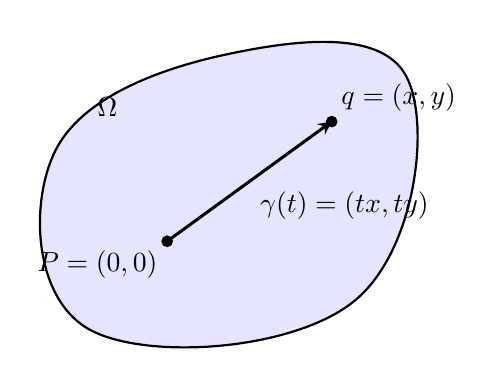
\begin{tikzpicture}[scale=0.95]
    \draw[thick, fill=blue!10] plot [smooth cycle, tension=0.7] coordinates {(-1,-1.2) (2.5,-0.8) (3.2,2.2) (0.8,2.5) (-1.5,1.2)};
    \coordinate (P) at (0,0);
    \coordinate (Q) at (2.2,1.6);
    \filldraw (P) circle (2pt) node[below left] {$P=(0,0)$};
    \filldraw (Q) circle (2pt) node[above right] {$q=(x,y)$};
    \draw[thick, line width=1.1pt, -stealth] (P) -- node[midway, below right] {$\gamma(t) = (tx, ty)$} (Q);
    \node at (-0.8, 1.8) {$\Omega$};
\end{tikzpicture}
\end{center}

Parametrize the line segment $\Gamma$ joining $P$ to $q$[cite: 1]:
\[
\gamma \colon [0, 1] \to \mathbb{R}^2, \quad \gamma(t) = (tx, ty), \quad \gamma'(t) = (x, y).
\]
Define the candidate potential function $f(x, y)$ by the line integral along $\Gamma$[cite: 1]:
\[
f(x, y) = \int_{\Gamma} F \cdot \mathrm{d}\ell = \int_0^1 F(\gamma(t)) \cdot \gamma'(t)\,\mathrm{d}t = \int_0^1 \big[ x F_1(tx, ty) + y F_2(tx, ty) \big]\,\mathrm{d}t.
\]
We now verify that $\nabla f = (F_1, F_2)$[cite: 1]. Differentiating with respect to $x$ under the integral sign[cite: 1]:
\[
\frac{\partial f}{\partial x} = \int_0^1 \left[ F_1(tx, ty) + tx \frac{\partial F_1}{\partial x}(tx, ty) + ty \frac{\partial F_2}{\partial x}(tx, ty) \right] \mathrm{d}t.
\]
Using the curl-free condition $\frac{\partial F_2}{\partial x} = \frac{\partial F_1}{\partial y}$[cite: 1]:
\[
\frac{\partial f}{\partial x} = \int_0^1 \left[ F_1(tx, ty) + tx \frac{\partial F_1}{\partial x}(tx, ty) + ty \frac{\partial F_1}{\partial y}(tx, ty) \right] \mathrm{d}t.
\]
By the multivariable chain rule, consider the derivative of $t \cdot F_1(\gamma(t))$ with respect to $t$[cite: 1]:
\[
\frac{\mathrm{d}}{\mathrm{d}t} \big( t \cdot F_1(tx, ty) \big) = F_1(tx, ty) + t \left[ \frac{\partial F_1}{\partial x}(tx, ty) \frac{\mathrm{d}(tx)}{\mathrm{d}t} + \frac{\partial F_1}{\partial y}(tx, ty) \frac{\mathrm{d}(ty)}{\mathrm{d}t} \right]
\]
\[
= F_1(tx, ty) + tx \frac{\partial F_1}{\partial x}(tx, ty) + ty \frac{\partial F_1}{\partial y}(tx, ty).
\]
Notice that the integrand of $\frac{\partial f}{\partial x}$ is exactly this total derivative:
\[
\frac{\partial f}{\partial x} = \int_0^1 \frac{\mathrm{d}}{\mathrm{d}t} \big( t \cdot F_1(tx, ty) \big)\,\mathrm{d}t = \Big[ t \cdot F_1(tx, ty) \Big]_{t=0}^1 = F_1(x, y) - 0 = F_1(x, y).
\]
By symmetry, applying the exact same differentiation with respect to $y$ gives[cite: 1]:
\[
\frac{\partial f}{\partial y} = F_2(x, y).
\]
Therefore, $\nabla f = (F_1, F_2) = F$, proving that $F$ derives from a scalar potential in $\Omega$[cite: 1]. \qed